\section{Diskrete Fourier-Transformation mit ANN\label{ml:dft-with-ann}}
\rhead{DFT mit ANN}

Die \emph{diskrete Fourier-Transformation} (DFT) einer Zahlenreihe $x_n \in \{ x_0, x_1, \cdots, x_{N-1}\}$
mit $N$ Elementen kann mit
\begin{equation}
    c_k = \frac{1}{N} \sum_{n=0}^{N-1} x_n e^{\normalsize -jk\frac{2\pi}{N}n}
\end{equation}
berechnet werden, oder in Vektorschreibweise
    \begin{equation}
    c_k = \begin{pmatrix}
        x_0\\
        x_1\\
        \vdots\\
        x_{N-1}
    \end{pmatrix} \cdot
    \frac{1}{N} \begin{pmatrix}
        e^{-j \omega_k 0} \\
        e^{-j \omega_k 1} \\
        \vdots \\
        e^{-j \omega_k (N-1)} \\
    \end{pmatrix}
    \qquad \text{mit}\qquad \omega_k = \frac{2\pi k}{N}.
    \label{ml:dft-with-ann:dft:vector}
\end{equation}
Die einzelnen $x_n$ werden mit einem komplexen Koeffizienten gewichtet und anschliessend
summiert. In der Vektorschreibweise wird dieser Effekt mit dem Skalarprodukt erzielt. Man
erkennt, dass dies ein linearer Zusammenhang ist.

Um uns auf die reellen Zahlen zu bschränken, wird \eqref{ml:dft-with-ann:dft:vector} in
die Kosinus-Anteile $a_k = 2{\rm Re}(c_k)$ und Sinus-Anteile $b_k = -2{\rm Im}(c_k)$
unterteilt:
\begin{equation}
    a_k = \vec x \cdot \frac{2}{N} \begin{pmatrix}
        1\\
        \cos(\omega_k 1)\\
        \vdots\\
        \cos(\omega_k (N-1))
    \end{pmatrix}
    = \vec x \cdot \vec \theta_{k,a}
    \quad \text{und} \quad
    b_k = \vec x \cdot \frac{-2}{N} \begin{pmatrix}
        0\\
        \sin(\omega_k 1)\\            
        \vdots\\
        \sin(\omega_k (N-1))
    \end{pmatrix}
    = \vec x \cdot \vec \theta_{k,b}.
\label{ml:dft-with-ann:dft:sin-and-cos-parts}
\end{equation}
Beide Teile sind bis auf die Koeffizienten genau gleich. Sie können  in der Form des mehrdimensionalen linearen
Modells \eqref{ml:ann:linear-unit} als
\begin{equation}
    \vec a = \begin{pmatrix}a_0\\ \vdots \\ a_{N-1} \end{pmatrix} = \begin{pmatrix}
        \vec \theta_{0,a} & \vec \theta_{1,a} & \cdots & \vec \theta_{N-1,a}
    \end{pmatrix} \vec x
    = {\bm \thetaup}_{a} \vec x
    \quad\text{und}\quad
    \vec b = {\bm \thetaup}_{b} \vec x
\label{ml:dft-with-ann:dft:sin-and-cos-parts:modell}
\end{equation}
geschrieben werden. Die konstanten Anteile entfallen.

In Abbildung~\ref{fig:ml:dft-with-ann:linear} ist das Netz für die Kosinus-Anteile abgebildet.
Als Übertragungsfunktion wurde für die Linearität die Identitätsfunktion $f(x) = x$ gewählt. Das Netz ist
also linear und nicht einmal affin (alle Bias-Werte sind Null). Ein analoges Netz kann
auch für die Sinus-Anteile erstellt werden. Alternativ können die Sinus-Koeffizienten aus
den Kosinus-Koeffizienten mit dem Zusammenhang
\begin{equation}
    \frac{N}{2} \arccos(\theta_{kn,a}) = \frac{N}{-2} \arcsin(\theta_{kn,b}) \quad \Leftrightarrow \quad
    \theta_{kn,b} = -\sin(\arccos(\theta_{kn,a}))
\end{equation}
berechnet werden.

\begin{figure}
    \centering
    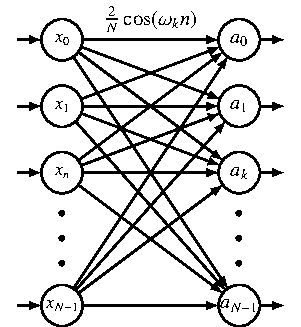
\includegraphics[scale=1]{papers/ml/images/ann_dft_linear.pdf}
    \caption{Lineares Netzwerk für die DFT.}
    \label{fig:ml:dft-with-ann:linear}
\end{figure}

Man kann erkennen, das so ein Netz unseren Fall der linearen Regression
(\ref{ml:regression}) exakt wiederspiegelt. Die Koeffizienten $\vec \theta_{k,a}$ und
$\vec \theta_{k,b}$ können also mit herkömmlichem Gradient-Descent gelernt werden, und das
sogar in endlich vielen Schritten, exakt. Um diese Aussage mit einem numerischen
Experiment nachzuprüfen, wurde das lineare Netz aus Abbildung \ref{fig:ml:dft-with-ann:linear}
wobei $N=1000$ mit \texttt{Keras} trainiert.
Abbildung~\ref{fig:ml:dft-with-ann:leanred-vs-dft} zeigt einen Vergleich der gelernten
Koeffizienten mit den Koeffizienten ${\bm \thetaup}_{a}$ und ${\bm \thetaup}_{b}$ der DFT.

Leider haben wir mit dieser Methodik überhaupt nichts gewonnen. Die Koeffizienten müssen
zwar nur \emph{einmal} gelernt werden bei gleichbleibendem $N$, um aber die
fouriertransformierten Werte $c_k$ zu berechnen, müssen immer noch zwei volle
Matrixvektormultiplikationen durchgeführt werden. Hier ist die schnelle
Fourier-Transformation bei weitem überlegen.
Die Frage, ob es möglich ist mit einem künstlichen neuronalen Netzwerk die Fourier-Transformation zu
berechnen können wir totzdem bejahen. Denn so ein lineares Netzwerk \emph{ist} ein FFANN,
wenn auch ein Spezialfall.

In einem weiteren numerischen Experiment wurde zuletzt versucht, mit einem dreischichtigen FFANN,
der $\tanh$-Aktivierungsfunktion und normalisierten Daten die DFT zu approximieren.
Auch nach einigem Testen von verschiedenen hyperparameter konnte kein befriedigendes
Ergebnis erbracht werden. Nur simple Eingangsdaten (zum Beispiel einfache
Schwingungen) konnten in guter Näherung transformiert werden.

Ein besserer Ansatz bietet \cite{ml:pmlr-v97-dao19a}, wobei durch ein speziell aufgebautes
lineares Netzwerk mit schwachbesetzten Schichten, Faktorisierungen\footnote{In
\ref{buch:diskret:subsetion:faktorisierung} ist eine Faktorisierung der
Fourier-Transformation und die daraus resultierende Reduktion der Anzahl Koeffizienten
beschrieben.} von einer Vielzahl der linearen Transformationen gelernt werden können.
\cite{ml:pmlr-v97-dao19a} zeigt also, dass ein vielschichtiges ANN mit geschicktem Aufbau in der Lage ist
einen fast beliebigen schnellen linearen Transformations-Algorithmus (zum Beispiel die FFT)
aus Daten zu rekonstruieren.

\begin{figure}
    \centering
    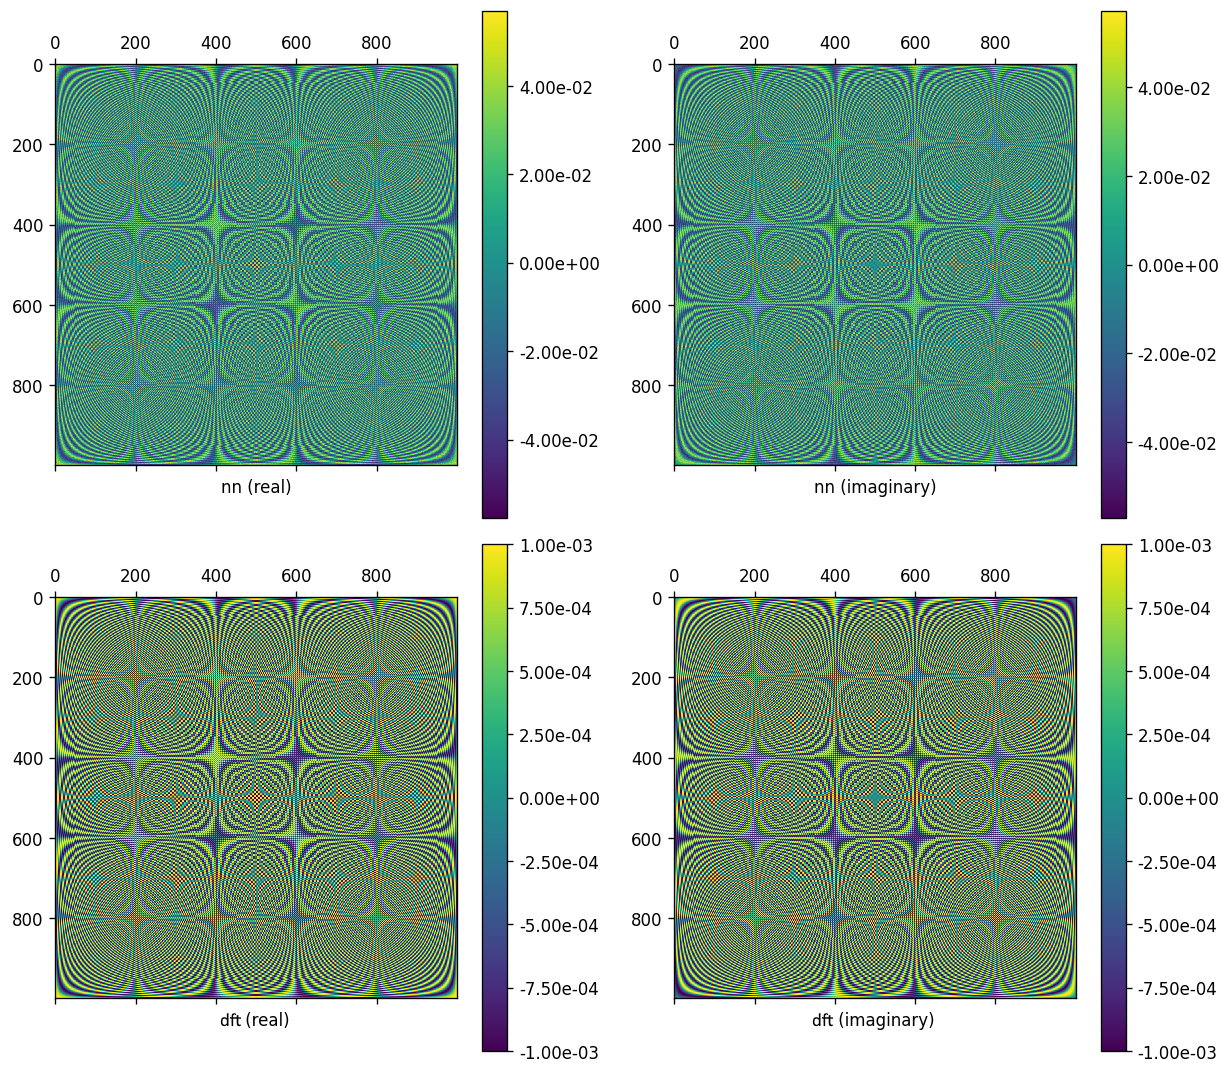
\includegraphics[width=\textwidth]{papers/ml/images/learned_coeff_vs_dft.png}
    \caption{Gelernte Koeffizienten-Matrix (oben) verglichen mit der DFT (unten).
    Beim trainieren des ANNs wurden normalisierte Daten verwendet, wodurch sich die
    Unterschiede erklären lassen.}
    \label{fig:ml:dft-with-ann:leanred-vs-dft}
\end{figure}
